\chapter{Monitorowanie procesu gojenia ścięgna Achillesa}
\section{Ścięgno Achillesa}
Ścięgno Achillesa, nazywane również ścięgnem piętowym, jest największym i zarazem wytrzymującym największe obciążenia ścięgnem występującym w ciele ludzkim. Stanowi wspólne zakończenie mięśnia trójgłowego łydki, w którego skład wchodzą dwie głowy mięśnia brzuchatego i mięsień płaszczkowaty. Całość struktury zlokalizowana jest w tylnym, powierzchownym przedziale łydki co zobrazowano na Rysunku \ref{muscle_structure}.  
\begin{figure}[h!]
\centering
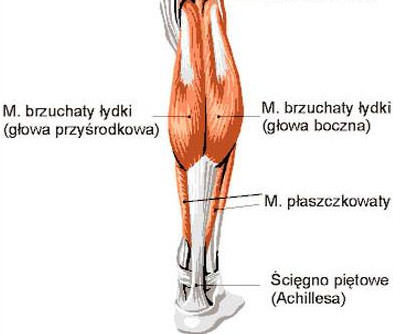
\includegraphics[width=0.55\textwidth]{figures/muscleStructure.jpg}
\caption{Lokalizacja mięśnia trójgłowego łydki wraz ze ścięgnem Achillesa.}
\label{muscle_structure}
\end{figure}

Procesy patofizjologiczne zachodzące po urazie ścięgna są ściśle związane z jego anatomią, biomechaniką, typem urazu i czynnikami jemu sprzyjającymi. Wszystkie te aspekty mają wpływ na możliwość monitorowania procesów gojenia się ścięgna i jego wspomagania, dlatego zostaną szczegółowo omówione w kolejnych podsekcjach. 

\subsection{Anatomia}

Z obu głów (brzuśców) mięśnia brzuchatego łydki wyrasta jedno szerokie, płaskie pasmo, które jest początkiem części brzuchatej ścięgna Achillesa. Następnie ścięgno to łączy się z włóknami pochodzącymi od mięśnia płaszczkowatego, które układają się stycznie do wcześniej powstałej struktury. Podążając w dół łydki, kształt ścięgna Achillesa ulega stopniowemu zwężeniu i zaokrągleniu, aż do punktu o minimalnej szerokości (około 4 cm nad przyczepem dolnym \cite{Doral2010}). W rejonie samego przyczepu, znajdującego się na guzie piętowym, ścięgno ponownie jest płaskie i szerokie.

Średnia długość ścięgna Achillesa to 15 cm (zakres to: 11 -- 26 cm). Średnia szerokość w rejonie początku wynosi 6,8 cm (4,5 -- 8,6 cm), w rejonie zwężenia to 1,8 cm (1,2 -- 2,6 cm), a w miejscu przyczepu dolnego 3,4 cm (2,0 -- 4,8 cm) \cite{Doral2010, KoivunenNiemel1995}.

Ścięgno jest zbudowane z tkanki łącznej, a dokładniej mówiąc z tkanki łącznej właściwej zbitej. Składa się w przeważającej części z \textit{istoty międzykomórkowej} (nazywanej też \textit{macierzą międzykomórkową}) zbudowanej z istoty podstawowej (ang. \textit{ground substance}) oraz włókien. Dopełnienie struktury stanowią komórki takie jak fibroblasty, komórki tuczne, komórki plazmatyczne, histiocyty i komórki napływowe. 

Istota podstawowa jest rodzajem żelu wiążącym duże ilości wody, włókien i komórek. Dokładniej mówiąc pełni ona rolę otoczki zapewniając możliwość transportu wody i substancji odżywczych do wnętrza struktury \cite{Sharma2006}, gdzie znajdują się komórki poukładane w wąskie pasy leżące pomiędzy włóknami \cite{Maffulli2005}. Wśród włókien można wyróżnić trzy rodzaje: kolagenowe, siateczkowe i sprężyste.

Włókna kolagenowe i siateczkowe są zbudowane z fibrylarnego białka -- kolagenu, najczęściej występującego białka w organizmie człowieka, stanowiącym około 25\% wszystkich białek. Makrocząsteczki kolagenu składają się ze zwiniętych łańcuchów polipeptydowych tworzących helisy. Dotychczas zidentyfikowano 20 typów kolagenu różniących się od siebie szczegółową budową helisy. Kolagen typu I stanowi około 90\% wszystkich typów i jest podstawowym budulcem włókien kolagenowych tworzących zazwyczaj wiązki o grubości 50--100$\mu$$m$. Włókna siateczkowe zbudowane są natomiast w przeważającym stopniu z kolagenu typu III. Pozostałe typy kolagenu występują w znacząco mniejszym stopniu tworząc włókienka kolagenowe i siateczkowe o różnej grubości -- od 10 do 300 nm (por. [Hist]).

Włókna sprężyste występują w postaci sieci i mają średnicę 0,2--10 $\mu$$m$. Zbudowane są z \textit{elastyny}, rozciągliwego i sprężystego białka. Dzięki temu włókna te pod wpływem działania siły zewnętrznej mogą zwiększać swoją długość nawet o 50\% (za. [Hist]). 

W strukturze zdrowego ścięgna Achillesa widoczne są ściśle upakowane włókna sprężyste i kolagenowe. Włókna kolagenowe stanowią 70\% masy suchego ścięgna i charakteryzują się hierarchiczną strukturą zobrazowaną na Rys. \ref{Achilles-histology}.  
\begin{figure}[h!]
	\centering
	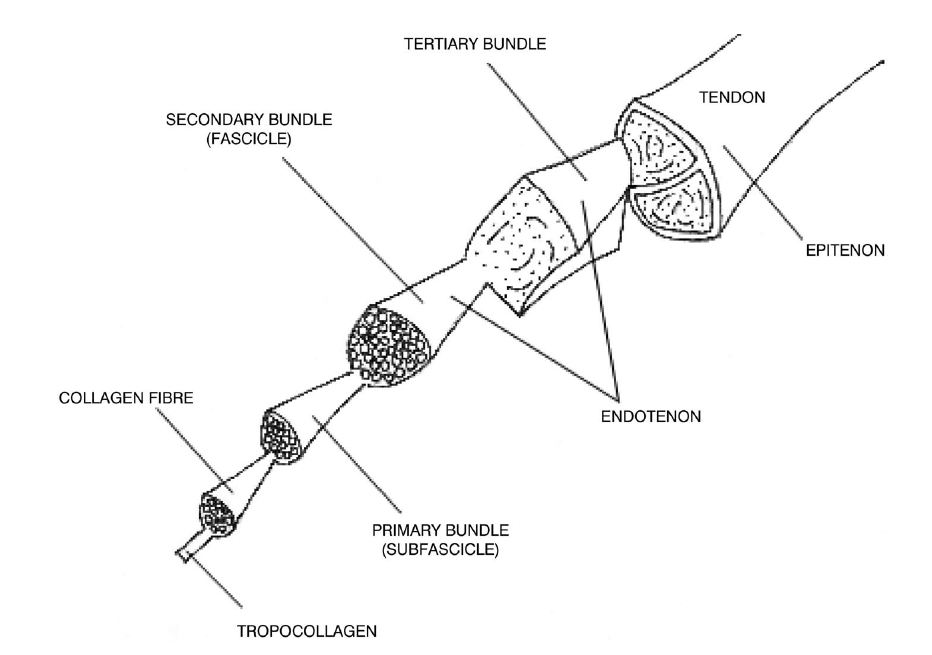
\includegraphics[width=0.8\textwidth]{figures/Achilles_hist.png}
	\caption{Schemat hierarchicznej budowy ścięgna Achillesa.}
	\label{Achilles-histology}
\end{figure}

Wyróżnić można: włókna, wiązki pierwszo, drugo i trzeciorzędowe oraz ościęgno \cite{Sharma2006}. W przeciwieństwie do innych ścięgien, ścięgno Achillesa nie posiada pochewki ścięgnistej, lecz jest otoczone ościęgnem utworzonym z tkanki łącznej włóknistej. Struktura ta jest bogata w naczynia krwionośne i jest bardzo ważnym elementem w procesie gojenia pełniąc funkcje transportowe. 

Oprócz otaczającej tkanki łącznej, ścięgno czerpie źródło unaczynienia z brzuśców mięśni brzuchatego i płaszczkowatego oraz z połączenia kostno-ścięgnistego. Najsłabsze unaczynienie występuje na poziomie ok. 4-5 cm powyżej górnego brzegu kości piętowej (por. \cite{bochenek2016anatomia}).

Unerwienie rejonu ścięgna Achillesa zapewniają nerw piszczelowy, biegnący wzdłuż całego ścięgna, a także nerw łydkowy, który krzyżuje się ze ścięgnem w odległości 8,7-12,4 cm proksymalnie od guza piętowego (por. \cite{bochenek2016anatomia}). 

\subsection{Biomechanika}
\label{Biomechanika}
Zadaniem ścięgien jest transfer siły mięśniowej do układu szkieletowego. Pod względem mechanicznym ścięgno piętowe jest najsilniejszym ścięgnem całego ustroju. Dla przykładu podczas chodu maksymalne obciążenie ścięgna Achillesa wynosi 500 N, przy biegu jest to 9000 N, natomiast podczas wyskoku może sięgać 12000 N, co stanowi równoważność 12--15 krotnej masy ciała. Podobne obciążenia wytrzymuje tylko ścięgno właściwe rzepki \cite{Etiologia}.

Głównym zadaniem ścięgna Achillesa w trakcie prawidłowego chodu, biegu, czy wyskoku jest ruch \textit{zginania podeszwowego stopy}, a zatem wyprost powodujący wspięcie na palce. Takie zadanie implikuje zwiększone ryzyko nadmiernego napięcia, a w konsekwencji przeciążenia, rozwoju stanu zapalnego, a nawet uszkodzenia ścięgna \cite{Etiologia}.

Cały proces ruchu rozpoczyna się od centralnego układu nerwowego skąd wysyłane są impulsy nerwowe. Trafiają one do odpowiednich grup mięśniowych za pośrednictwem \textit{nerwu ruchowego}, struktury  przewodzącej impulsy wzbudzające proces skurczu mięśni. Na styku nerwu z mięśniem znajduje się \textit{synapsa nerwowo-mięśniowa} (tzw. \textit{płytka motoneuronalna}). Do niej właśnie na skutek impulsu wydzielany jest neuroprzekaźnik, \textit{acetylocholina}. W wyniku działania tej substancji następuje dalsze pobudzenie błony komórki mięśniowej i uwolnienie jonów wapnia Ca$^{2+}$. Cząsteczki te aktywują białka kurczliwe tj. \textit{aktynę} i \textit{miozyną}, a także pośrednio wywołują produkcję w mięśniu \textit{adenozyno-5'-trifosforanu, ATP}, czyli substancji zapewniającej dostarczenie odpowiedniej energii chemicznej dla procesu.

Cały proces pobudzenia skurczu, dla mięśni szkieletowych trwa 100--300 milisekund. Schemat czasów poszczególnych aktywacji przedstawiono na Rys. \ref{muscle-excitements}. 
\begin{figure}[h!]
	\centering
	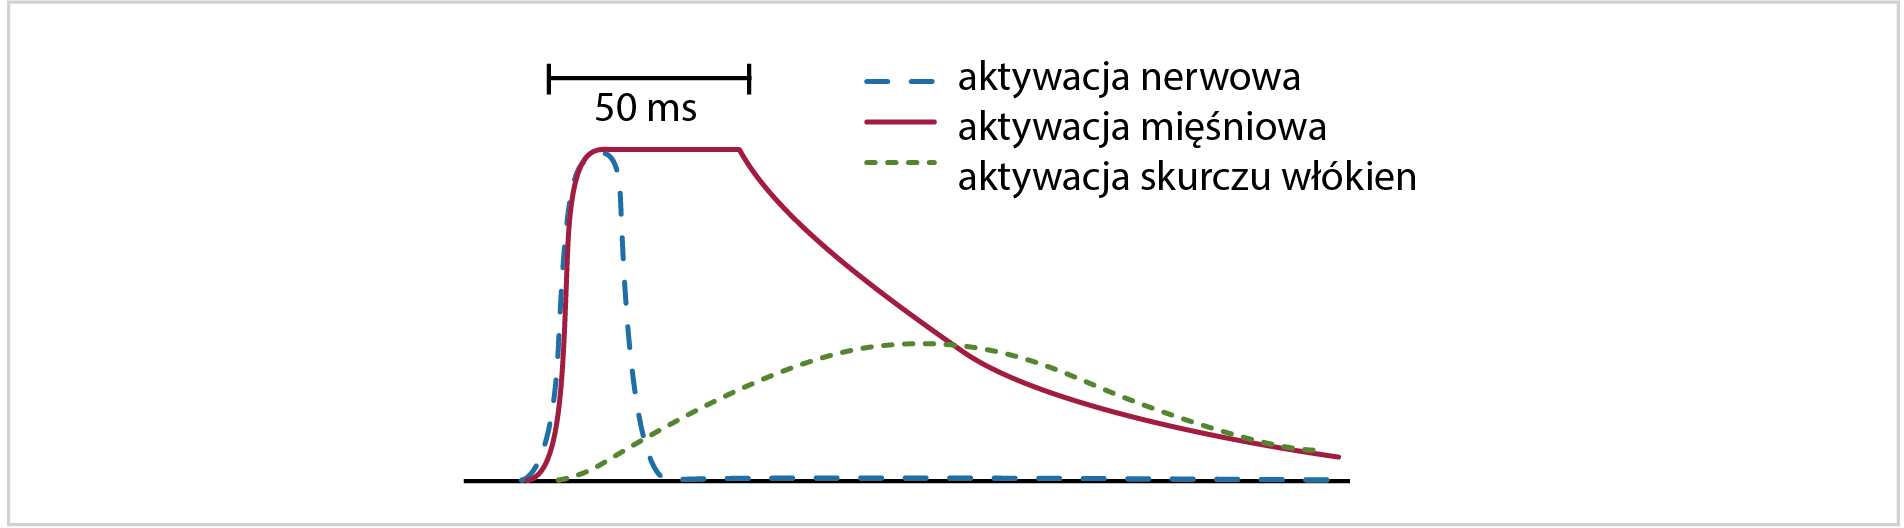
\includegraphics[width=0.6\textwidth]{figures/skurcz_miesni.png}
	\caption{Schemat generowania skurczu mięśni.}
	\label{muscle-excitements}
\end{figure}

Jak wcześniej zaznaczono, siła wygenerowana przez skurcz jest przekazywana za pomocą ścięgien do układu szkieletowego. Dobrym przybliżeniem tego procesu jest \textit{model Hill'a} \cite{Hill1938}, którego schemat przedstawiono na Rys. \ref{hill-model}.

\begin{figure}[h!]
	\centering
	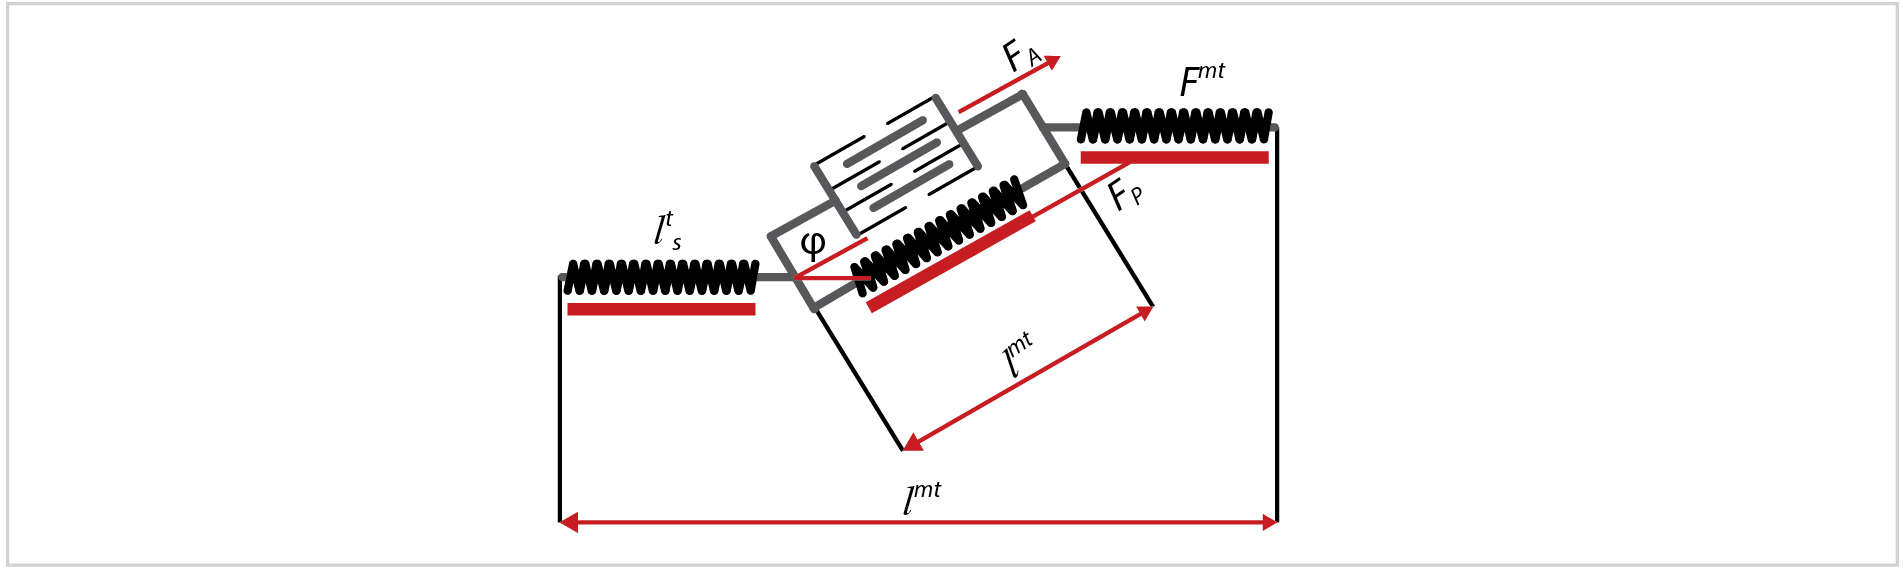
\includegraphics[width=0.6\textwidth]{figures/Hill.png}
	\caption{Schemat modelu Hilla.}
	\label{hill-model}
\end{figure}

Gdzie $F_A$ oznacza siłę aktywnie wywoływaną skurczem mięśni, $F_P$ to pasywna siła odpowiadająca za bezwładność tkanki miękkiej w mięśniu, a $F^{mt}$ to wynikowa siła przekazywana przez ścięgno, która zależy od długości ścięgna $l_t$ i kąta $\phi$ pomiędzy ścięgnem a mięśniem. 

To właśnie na skutek przekroczenia wartości granicznej siły $F^{mt}$ dochodzi najczęściej do urazu ścięgna Achillesa. Dokładny opis tego problemu wraz z jego implikacjami został przedstawiony w kolejnej podsekcji.

\subsection{Urazy i czynniki im sprzyjające}

Uszkodzenie ścięgna Achillesa uznawane jest obecnie za chorobę cywilizacyjną (za \cite{Etiologia}). Przykładowo, dla społeczeństwa amerykańskiego, urazy te występują u 18 na 100.000 osób rocznie \cite{EpidemiologyUS}. Dodatkowo ryzyko ponownego zerwania ścięgna wynosi 20--40\% \cite{EpidemiologyUS}. 

Można wyróżnić dwa mechanizmy uszkodzenia ścięgna Achillesa: 
\begin{enumerate}
	\item uraz bezpośredni -- do którego zaliczyć można otwarte urazy spowodowane np. przecięciem ostrym przedmiotem takim jak szkło oraz urazy zamknięte spowodowane nagłym uderzeniem w napięte ścięgno.
	\item uraz pośredni -- znacznie częściej spotykany niż uraz bezpośredni. Powstaje w wyniku nagłego, silnego skurczu mięśnia połączonego często z innymi siłami zewnętrznymi towarzyszącymi np. upadkowi.
\end{enumerate}
O ile uraz bezpośredni jest najczęściej następstwem nieszczęśliwego wypadku, o tyle urazy pośrednie mają swoją przyczynę w rodzaju wykonywanych czynności oraz predyspozycji danej osoby. 

Najczęściej do tego rodzaju urazów dochodzi podczas uprawiania sportu. Dotyczy to zwłaszcza sportu rekreacyjnego (około 70\% przypadków \cite{EpidemiologyUS, Etiologia}).
Aż 75\% przypadków przytrafia się mężczyznom w przedziale wiekowym wahającym się od 30 do 50 roku życia \cite{Etiologia}. Statystyki te mają związek z obniżeniem poziomu ukrwienia ścięgna po 30 roku życia i trybem życia związanym ze sporadycznym, ale nadmiernym obciążaniem ścięgna przez osoby niewytrenowane \cite{Etiologia}. 

Dyscypliny sportowe, podczas których najczęściej dochodzi do urazu ścięgna Achillesa to: piłka nożna, siatkówka, tenis, taniec, koszykówka, skoki, biegi, piłka ręczna, aerobic, pływanie, ping-pong, biegi, narciarstwo, balet. Proporcje są naturalnie uzależnione od popularności danego sportu w konkretnym kręgu ludzi. Dla przykładu na Rys. \ref{rupture} zobrazowano udział poszczególnych dyscyplin w urazach ścięgna Achillesa dla amerykańskiego społeczeństwa \cite{EpidemiologyUS}. 

\begin{figure}[h!]
	\centering
	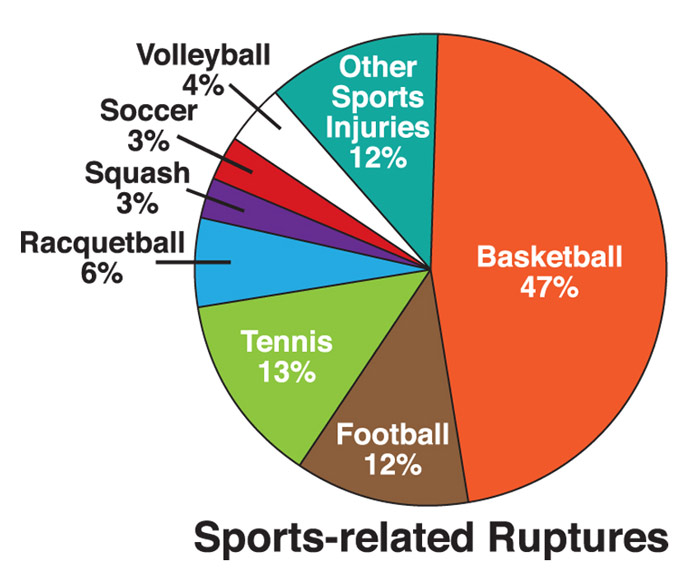
\includegraphics[width=0.6\textwidth]{figures/Achilles_zerwanie.jpg}
	\caption{Wykres przedstawiający proporcje występowania urazu ścięgna Achillesa w różnych dyscyplinach sportowych na przykładzie amerykańskiego społeczeństwa.}
	\label{rupture}
\end{figure}
W Stanach Zjednoczonych sportem największego ryzyka jest koszykówka, natomiast w Europie jest to piłka nożna (około 60\%). Według szacunków przedstawionych w \cite{CHIRALI2014211} uraz ścięgna Achillesa stanowi 5--10\% wszystkich urazów atletycznych.

Powszechnie uważa się, że zdrowe ścięgno piętowe jest bardzo ciężko zerwać z uwagi na jego dużą wytrzymałość. Dla przykładu wycinek ścięgna o przekroju 1 cm$^2$ jest w stanie utrzymać masę 500--1000 kg \cite{Maquirriain2011}. Do urazów dochodzi zatem najczęściej, gdy ścięgno jest zmienione patologicznie. Czynniki powodujące osłabienie ścięgna Achillesa można podzielić na: zewnętrzne i wewnętrzne.

Do czynników wewnętrznych należy zaliczyć:
\begin{itemize}
	\item mechaniczne uszkodzenie ścięgna -- uraz bezpośredni (np. częściowe przecięcie);
	\item zmiany degeneracyjne -- inwolucyjne (wiek powyżej 30 roku życia), na podłożu stanów zapalnych (przewlekłe stany zapalne), związane z mikrourazami;
	\item nadmierne przeciążenia -- nieprawidłowa aktywność fizyczna;
	\item choroby metaboliczne i układowe -- takie jak np. toczeń trzewny, dna moczanowa, nadczynność tarczycy, gruczolaki przysadki mózgowej, reumatoidalne zapalenie stawów, kolagenozy;
	\item odchylenia anatomiczne i biomechaniczne -- anomalie takie jak: piszczel szpotawa, stopa koślawa, stopa płasko-koślawa, niestabilność stawu skokowego, koślawość lub szpotawość tyłostopia, osłabienie i przykurcz mięśni okołostawowych, ograniczenie ruchomości stawu skokowo-goleniowego i skokowo-piętowego, nierówność kończyn dolnych, nieprawidłowy stereotyp chodu, pogłębione krzywizny kręgosłupa, zespół ciasnoty przedziałów powięziowych w obrębie przedziału tylnego goleni;
	\item zaburzenia naczyniowe -- schorzenia takie jak: hyperlipidemia, cukrzyca lub wywołane nadmiernym paleniem tytoniu;
	\item dysbalans mięśniowy;
	\item zaburzenia proprioceptywne;
	\item niepełne wyleczenie poprzednich obrażeń;
	\item przyjmowanie kortykosteroidów;
\end{itemize}

Do czynników zewnętrznych zaliczyć można:
\begin{itemize}
	\item błędy w metodyce prowadzenia zajęć -- np. nadmierny trening, trening jednostronny, trening wszechstronny, z przewagą intensywności nad wytrzymałością czynnościową aparatu więzdłowo-stawowo-mięśniowego, chęć nadrobienia zaległości treningowych;
	\item nagła zmiana dyscypliny sportowej lub aktywności rekreacyjnej;
	\item inne takie jak: nieodpowiednia nawierzchnia, niekorzystne warunki pogodowe, nieodpowiednie obuwie, zbyt krótkie przerwy między zawodami lub treningami.
\end{itemize}

Obecnie, ustalenie jednej optymalnej metody leczenia dla każdego rodzaju uszkodzenia ścięgna Achillesa nie jest możliwe. Wybór uwarunkowany jest poziomem i stopniem zniszczenia ścięgna, stanem zdrowia pacjenta oraz kwalifikacjami, doświadczeniem i możliwościami danego ośrodka. W kolejnej sekcji omówione zostaną współczesne metody leczenia tego schorzenia, natomiast w Rozdziale [] zaprezentowana zostanie nowa metoda monitorowania procesu gojenia się ścięgna Achillesa, która może być wykorzystana do optymalizacji rehabilitacji opisanego problemu. 

\subsection{Fazy gojenia, leczenie i rehabilitacja}
\label{gojenie}

Proces gojenia się ścięgna Achillesa można podzielić na trzy zachodzące na siebie etapy. W pierwszej kolejności dochodzi do stanu zapalnego. Jest to tzw. \textit{faza zapalna} (ang. \textit{inflammatory phase}), która trwa w pierwszym tygodniu gojenia się. Następnie występuje \textit{faza proliferacji} (ang. \textit{proliferative phase}), trwająca od drugiego do szóstego tygodnia. Cały proces kończy się \textit{fazą przebudowy} (ang. \textit{remodeling phase}), która może trwać nawet do 18 miesiąca po urazie \cite{Sharma2006, Yang2013, Docheva2015, CMC}. 

Faza zapalna zaczyna się od razu po wypadku. W miejscu urazu tworzy się skrzep krwi oraz uwalniane są prozapalne substancje chemiczne, cytokiny, które w znaczącym stopniu odpowiadają za proces aktywacji i migracji komórek zapalnych z otoczenia do miejsca zapalenia \cite{Lin2004}. Komórki te, a dokładniej mówiąc leukocyty i makrofagi, rozpoczynają \textit{fagocytozę}, czyli proces mający na celu usunięcie obumarłej tkanki oraz skrzepu \cite{Yang2013, Beredjiklian2003, Lin2004}. Symultanicznie dochodzi do aktywacji i selekcji \textit{tenocytów} (komórek ścięgna), które rozpoczynają odbudowę włókien ścięgna \cite{Yang2013} oraz inicjują drugą fazę całego procesu.

W fazie proliferacji poziom komórek zapalnych zaczyna spadać. Czynniki wzrostu, uwalniane m.in. przez makrofagi, nasilają migrację i rozmnażanie się tenocytów wokół miejsca urazu. Skutkiem tego jest wytworzenie nowych włókien kolagenu typu III. Nowo-powstałe struktury są początkowo losowo zorientowane \cite{Yang2013, Beredjiklian2003, Docheva2015}. Dlatego rozpoczyna się trzecia faza mająca na celu odtworzenie struktury zdrowego ścięgna.

W trakcie trwania ostatniej fazy, nazywanej również \textit{remodelingiem} włókna kolagenu typu III zastępowane są kolagenem typu I. Pod wpływem naprężeń struktura włókien zmienia się i wyrównuje zgodnie z kierunkiem występujących sił \cite{Yang2013}. Włókna pracujące niezgodnie z przewidzianym ruchem ulegają zerwaniu i fagocytozie, a te które wspomagają zadany ruch ulegają wzmocnieniu. 

Pomimo całego wyżej opisanego procesu ścięgno wygojone strukturą odbiega od ścięgna zdrowego. Charakteryzuje się nawet dwukrotnie zwiększoną powierzchnią przekroju osiowego, podatnością na ponowne zerwania z uwagi na zmniejszoną odporność na obciążenia. 

Uraz ścięgna Achillesa można leczyć zachowawczo lub operacyjnie. Zachowawcze leczenie stosuje się najczęściej przy częściowym uszkodzeniu ścięgna lub u osób, które mają przeciwwskazania do leczenia chirurgicznego. Wówczas stosowane jest unieruchamianie kończyny np. poprzez włożenie w but ortopedyczny lub gips. Dodatkowo można również stosować preparaty z komórek macierzystych i czynników wzrostu \cite{CMC}. Wybór leczenia zachowawczego wiąże się z długotrwałym, trwającym około 10 tygodni unieruchomieniem kończyny przed przystąpieniem do rehabilitacji.

Leczenie operacyjne stosowane jest najczęściej w przypadku uszkodzenia całkowitego. Tuż po urazie lub po przejściu najintensywniejszych procesów fazy zapalnej wykonuje się szycie ścięgna. Stosowane są metody operacji na otwartym ścięgnie lub przeźskórnie. Zabieg przezskórny polega na zbliżeniu kikutów ścięgna specjalnym szwem przeprowadzanym przez małe nacięcia. W teorii metoda ta umożliwia szybsze obciążanie nogi po operacji, skraca okres unieruchomienia i umożliwia szybszą rehabilitację. W praktyce jednak chirurgom rzadko udaje się uzyskać jakość zszycia porównywalną z metodą otwartą. 

Rehabilitacja po urazie również podzielona jest ze względu na fazy gojenia. W pierwszej fazie terapia skupia się wokół ochrony miejsca urazu, odciążenia nogi, redukcji obrzęku i złagodzenia stanu zapalnego. Dokonuje się również zabiegów mających na celu wczesną mobilizację ścięgna i przywrócenia ślizgu. Ochrona miejsca urazu może być wykonana przez zastosowanie dwu-częściowej łuski gipsowej lub buta ortopedycznego. Redukcję obrzęku wykonuje się poprzez np. masaż limfatyczny. Stan zapalny łagodzony jest chłodzeniem i okładami oraz lekami, natomiast ślizg przykładowo stymuluje się przez elektrostymulacje oraz mobilizacje mięśni łydki poprzez zginanie stopy.

W drugiej fazie zabiegi rehabilitacyjne są kontynuacją działań wykonywanych podczas pierwszej fazy. Szczególny nacisk przewidziany jest na przeciwdziałanie powstawania zrostów poprzez pracę nad ślizgiem ścięgna oraz mobilizacją tkanek miękkich. W szczególności rehabilitanci poświęcają dużo uwagi na ćwiczenia dotyczące mobilizacji blizny i tkanek okalających. Nasilane są również zabiegi związane z elektrostymulacją celem utrzymania masy mięśniowej oraz wykonywane są ćwiczenia związane ze stabilizacją stawu skokowego związane z ćwiczeniami izometrycznymi mięśni prostujących i pronujących stopę. W tej fazie stosuje się wciąż ochronę miejsca urazu oraz aplikuje się metody redukcji obrzęku.

Trzeci etap tj. przebudowa to najdłuższy z etapów gojenia się tkanek ścięgnistych, podczas którego zachodzi najwięcej zmian w strukturze, odporności ścięgna oraz jego funkcji. W tym okresie można wyszczególnić następujące cele rehabilitacji: 
\begin{itemize}
	\item przeciwdziałanie zrostom tkanek otaczających Achillesa; 
	\item wzmocnienie mięśni łydki – brzuchatego i płaszczkowatego; 
	\item przywrócenie pełnego zakresu ruchu i kluczowych funkcji ścięgna; 
	\item zwiększenie elastyczności tkanek wokół ścięgna;
\end{itemize}

Oprócz podstawowych zabiegów ochronnych i fizjoterapii do działań włączane są terapie związane z ćwiczeniami czynnymi z oporem; stymulujące technikę prawidłowego chodu; ćwiczenia wzmacniające obręcz biodrową; ćwiczenia sensomotoryczne w różnych pozycjach ciała oraz ćwiczenia wzmacniające kończyny dolne na niestabilnym podłożu. Powoli wprowadzane są również aktywności sportowe takie jak rower stacjonarny czy stretching. Celem finalnym tego etapu jest powrót do pełnej sprawności. 

Dużą nadzieję wiążę się z nowymi technikami bazującymi na zastrzykach z komórek macierzystych. Ciekawą propozycją wydaje się możliwość budowania biodegradowalnych rusztowań (ang. \textit{scaffold}), implementowanych podczas operacji i wspomagających implementację komórek macierzystych i czynników wzrostu w odpowiednie miejsca \cite{START}.

Celem oceny tego rodzaju nowatorskich podejść jak również z uwagi na konieczność optymalizacji istniejących metod rehabilitacji i leczenia urazów ścięgna Achillesa potrzebne jest monitorowanie procesu gojenia. Najczęściej stosowane techniki zostaną omówione w kolejnych sekcjach.

\section{Zastosowanie rezonansu magnetycznego}
 
Obserwację gojącej się struktury ścięgna Achillesa umożliwiają techniki stosujące różnego rodzaju fale przenikające ciało ludzkie. W zależności od wyrażanej w hercach (w skr. Hz) \textit{częstotliwości fali}, czyli liczby pełnych cykli drgań w ciągu sekundy oraz \textit{amplitudy} tj. maksymalnej wartości sygnału, fala rozchodzi się w ośrodku implikując różne możliwe do interpretacji zdarzenia wykorzystywane w technikach obrazowania medycznego. 

Pierwszą opisaną w tej pracy metodą obrazowania stosowaną do monitorowania gojenia się ścięgna Achillesa jest obrazowanie z wykorzystaniem \textit{Jądrowego Rezonansu Magnetycznego} nazywanego dla uproszczenia \textit{Rezonansem Magnetycznym}, w skr. \textit{RM}. Metoda ta bazuje na odpowiednim odczycie reakcji jąder atomów na stałe pole magnetyczne generowane przez magnesy, zmienne pole magnetyczne skierowane prostopadle do osi stałego pola (generowane w dedykowanej do tego zadania cewce), zmienne pole lokalne wytwarzane przez sąsiednie jądra atomowe oraz związane z nimi cząstki elementarne.

Zrozumienie własności jądra atomowego i reakcji na magnetyzację było możliwe dzięki badaniom naukowym z początku XX wieku. Zapewniły one praktyczną możliwość wykorzystania procesów bazujących na zachowaniach obiektów o bardzo małych masach i wymiarach takich jak cząstki elementarne. Jako przykłady można wskazać prace Alberta Einsteina dotyczące ruchów Browna oraz efektu fotoelektrycznego; opis funkcji falowej zaproponowany przez Erwina Shrodingera; badania Nielsa Bohra, które doprowadziły do utworzenia utylitarnego modelu atomu zawierającego poziomy energetyczne; wyprowadzenie reguły nieoznaczoności przez Werner Heisenberga, czy opisanie przez Wolfganga Pauliego konfiguracji cząstek elementarnych w atomie. 

W dużej mierze na bazie powyższych prac zdefiniowana została teoria mechaniki kwantowej umożliwiająca pogłębienie wiedzy na temat magnetycznej natury składników jądra atomowego tj. \textit{protonów} i \textit{neutronów}. Pierwszy ważny przełom nastąpił w 1933 r., kiedy to Frisch i Stern w \cite{Frisch1933} opisali moment magnetycznego protonu. Rok później, w \cite{Breit1934} Breit i Rabi zaproponowali metodę rezonansową obserwacji własności magnetycznych jąder atomowych. W 1946 praca ta została udoskonalona i wykorzystana przez Felix Bloch'a do badania cząstek w wodzie i parafinie \cite{Bloch1946}. W końcu dzięki pracom m.in. Lautenrbur'a \cite{LAUTERBUR1973} i Mansfield'a \cite{Mansfield1977} rozwinęły się metody lokalizacji przestrzennej powyższych zmian własności magnetycznych, co umożliwiło utylitarną prezentację wizualną wyników. 

Opisując zagadnienie dokładniej, należy zwrócić uwagę na główną własność jądra atomowego umożliwiającą działanie RM, czyli \textit{spin}. Można powiedzieć, że jądro posiada spin jeżeli nie ma jednocześnie parzystej liczby protonów i neutronów (za \cite{RM2015}). Dla przykładu jądro wodoru składające się z 1 protonu spełnia powyższy warunek. 

Umieszczone w polu magnetycznym jądra atomowe posiadające spin wykonują ruch wirowy zwany \textit{precesją}. Częstotliwość tej precesji jest proporcjonalna do natężenia pola magnetycznego i opisana jest \textit{równaniem Larmora} \ref{MRLarmor}:
\begin{equation}
\label{MRLarmor}
\omega_0 = \gamma \ast \beta_0,
\end{equation}
gdzie $\omega_0$ to prędkość obrotowa protonów (tzw. \textit{częstotliwość Larmora}), $\gamma$ to współczynnik żyromagnetyczny właściwy danemu protonowi, a $\beta_0$ to wartość natężenia danego pola magnetycznego. Dla przykładu częstotliwość Larmora dla protonu wodoru, gdzie $\gamma$=42,57 MHz/T dla pola 1,5T równa jest 63,8 MHz. 

Jądra atomowe wirujące z częstotliwością Larmora ulegają swego rodzaju uporządkowaniu, tworząc rotujące tak samo wektory magnetyzacji. Dodatkowo, istotne jest, że wektory te stowarzyszone z jądrami o wysokich poziomach energii odchylają się przeciwnie do zwrotu pola magnetycznego -- antyrównolegle, a o niskich poziomach energii odchylają równolegle, czyli zgodnie ze zwrotem pola magnetycznego. W przeciętnym wycinku ciała ludzkiego jest znacząco więcej jąder o ustawieniu równoległym niż antyrównoległym. Przykładowo w objętości 1 $\times$ 1 $\times$ 5 mm jest to liczba około 2 $\times$ $10^{15}$ cząstek. Różnica ta tworzy całkowitą magnetyzację $M_0$ danego obszaru, która wyjściowo ma większą wartość zgodną ze zwrotem pola magnetycznego, czyli tzw. \textit{magnetyzacji podłużnej}. Kierunek prostopadły do magnetyzacji podłużnej nazywany jest \textit{magnetyzacją poprzeczną}.

Zmiana $M_0$ obszaru, tworzy sygnał MR. Wykonuje się ją przy pomocy odpowiednio sterowanej cewki nadającej impulsy o częstotliwości fal radiowych (tzw. \textit{impulsy RF} -- od ang. \textit{Radio Frequency}). Impuls RF jest krótkotrwały i ma taką samą częstotliwość, co częstotliwość precesji. Dzięki temu zachodzi zjawisko \textit{rezonansu magnetycznego}, czyli wymiany energii między jądrami atomowymi, a falą radiową. Cząstka pochłania wówczas energię \textit{fotonu}, tj. nośnika oddziaływania elektromagnetycznego, i uzyskuje wyższy poziom energetyczny, odchylając wektor magnetyzacji i zaburzając tym samym uporządkowanie. Następuje zmniejszenie $M_0$ w kierunku podłużnym oraz wzrost magnetyzacji poprzecznej. Po wyłączeniu impulsu RF magnetyzacja wraca do wartości początkowej. Czas potrzebny na zwiększenie magnetyzacji podłużnej do stanu z przed działania impulsu nazywany jest czasem \textit{relaksacji podłużnej}, \textit{relaksacji spin -- sieć} lub \textit{czasem T1}. Natomiast czas potrzebny na obniżenie magnetyzacji poprzecznej nazywany jest czasem \textit{relaksacji poprzecznej}, \textit{relaksacji spin – spin} lub \textit{czasem T2}.  

Lokalizacja zmian magnetyzacji w poszczególnych \textit{wokselach} (tj. wycinkach przestrzeni 3D o określonych wymiarach) odbywa się przy pomocy celowanego różnicowania fazy i częstotliwości wektorów magnetyzacji w odpowiednich obszarach. Odbywa się to przy pomocy sygnału z dodatkowych cewek gradientowych. Warstwa, w której dokonywany jest pomiar kodowana jest przy pomocy nałożenia na pole $\beta_0$ pola gradientowego $G_{zz}$, co umożliwia wzbudzenie jąder atomowych w tych wokselach, dla których współrzędna $z$ wyraża się wzorem:
\begin{equation}
\Delta z = \frac{\Delta \omega}{\gamma G_{zz}},
\end{equation}
gdzie $\Delta \omega$ to szerokość widmowa pobudzającego jądra impulsu RF. Współrzędna $y$ kodowana jest przy pomocy zróżnicowania fazy rotujących w różnych obszarach wektorów magnetyzacji na skutek działania pola gradientowego $G_{yz}$ — tzw. \textit{gradientu kodowania fazy}. Zróżnicowanie to wyraża się wzorem:
\begin{equation}
\phi = \gamma G_{yz}yT_{y},
\end{equation}
gdzie $T_y$ oznacza czas włączenia pola gradientowego $G_{yz}$. Ostatecznie włączany jest gradient $G_{xz}$ w wyniku czego następuje zróżnicowanie częstości precesji wektora magnetyzacji w kolejnych wokselach (zob. [https://brain.fuw.edu.pl/edu/index.php/]). 

Nieprzetworzona informacja z wokseli o współrzędnych $x$, $y$, $z$ nazywana jest \textit{przestrzenią K} i koduje ona składniki częstotliwości sygnału RM. Do transformacji z przestrzeni częstotliwości na przestrzeń obrazu używana jest operacja matematyczna zwana \textit{odwrotną transformacją Fouriera}. Przykład takiego działania można znaleźć w [http://mriquestions.com/fourier-transform-ft.html].

Z uwagi na różne parametry mierzone w reakcji protonów na zadane pole magnetyczne powstało wiele \textit{sekwencji MR} oraz ich składowych nazywanych w tej pracy \textit{protokołami MR}. Do badań opisanych w dalszej części tego manuskryptu zostało użytych 10 często spotykanych wariantów pracy rezonansu magnetycznego. Zostaną one pokrótce scharakteryzowane poniżej:
\begin{itemize}
	\item \textit{T1} -- mierzona jest \textit{relaksacja T1}, a zatem czas potrzebny protonom na powrót do stanu początkowego po odchyleniu o 90$^\circ$. Sygnał rezonansu magnetycznego $MR_s$ można obliczyć z zależności:
	\begin{equation}
		MR_s \sim \gamma_{pd} \ast [1-e^{-TR/T1}],
	\end{equation}
	gdzie $\gamma_{pd}$ to gęstość protonowa tkanki, $TR$ to \textit{czas repetycji} określany przez użytkownika.
	\item \textit{T2} -- mierzona jest \textit{relaksacja T2}, tj. czas potrzebny do utraty spoistości pomiędzy spinami. Dokładniej mówiąc mierzone są różnice w częstotliwości Larmora powstające w czasie, wynikające z umiejscowienia protonów w różnych ośrodkach i niejednorodności w pobudzeniach polem magnetycznym. $MR_s$ przyjmuje wówczas następującą zależność:
	\begin{equation}
	\label{T2ecquation}
	MR_s \sim \gamma_{pd} \ast [1-e^{-TE/T2}],
	\end{equation}
	gdzie $TE$ to \textit{czas echa} zdefiniowany przez użytkownika.
	\item \textit{PD} (od ang. \textit{Proton Density}) -- mierzona jest gęstość spinowa tkanki wprost proporcjonalna do liczby protonów. Wówczas:
	\begin{equation}
	MR_s \sim \gamma_{pd}.
	\end{equation}
	\item \textit{T2 mapping} -- $T2$ z sygnału \ref{T2ecquation} mierzona jest dla wielu $TE$, co pozwala na interpolacje między wynikami z własnym doborem parametrów (zob. [Regulski]).
	\item \textit{T2 $^\ast$ GRE} (od ang. \textit{Gradient Echo}) -- jest to przykład \textit{sekwencji gradientowych}. W sekwencjach gradientowych protony odchylane są o kąt mniejszy od $90^\circ$ (zazwyczaj 10$^\circ$ -- 80$^\circ$). Odchylenia protonów występują z określoną częstotliwością prowadząc do cyklicznego przefazowania spinów. Dzięki temu uzyskuje się skupione echo gradientowe w czasie $TE$, w którym sygnał $MR_s$ jest zależny od obu czynników $T1$ i $T2$:
	\begin{equation}
	MR_s \sim \gamma_{pd} \ast [1-e^{-TE/T2}][1-e^{-TR/T1}],
	\end{equation}
	przy czym dla mniejszych kątów wkład $T2$ rośnie w stosunku do wkładu $T1$.
	\item \textit{T2 $^\ast$ GRE TE\_MIN} (od ang. \textit{Minimal Time Echo}) -- mierzone jest $T2$ z sygnału \ref{T2ecquation} przy minimalnym czasie $TE$ i tylko dla fragmentu przestrzeni K. 
	\item \textit{3D FSPGR} (od ang. \textit{Fast Spoiled Gradient Echo}) -- jest to szybka sekwencja gradientowa, wykorzystująca echo szczątkowe oraz \textit{spoiler}, tj. metodę do rozbicia wszelkiej pozostałej magnetyzacji na końcu każdego cyklu przefazowania. W tej pracy użyto czterech protokołów tej sekwencji. Wszystkie bazują na różnicy w częstotliwościach rezonansowych protonów wchodzących w skład tłuszczu i wody oraz przesunięciach fazowych wynikających z tych różnic. Dokładniej:
	\begin{itemize}
		\item In Phase Ideal -- sygnał mierzony w czasie, gdy protony należące do tłuszczu i wody są w zgodnej fazie;
		\item Out Phase Ideal -- sygnał mierzony w czasie, gdy protony należące do tłuszczu i wody są w antyfazie;
		\item Fat Ideal -- sygnał mierzony przy maksymalnej wartości fazy protonów tłuszczu i minimalnej protonów wody;
		\item Water Ideal -- sygnał mierzony przy maksymalnej wartości fazy protonów wody i minimalnej protonów tłuszczu.
	\end{itemize}
\end{itemize}

Wodór jest najczęściej wykorzystywanym pierwiastkiem w metodzie rezonansu magnetycznego, gdyż jest obecny w 99,98\% ludzkich tkanek (za [MR]). Jednak w szczególnych przypadkach stosuje się również obrazowania z wykorzystaniem częstotliwości odpowiednich dla fosforu, sodu czy węgla (zob. []).

Rezonans magnetyczny może być wykorzystany do monitorowania gojenia się ścięgien i więzadeł, gdyż tkanki miękkie człowieka składają się w największej części z atomów wodoru. W szczególności umożliwia to obserwację: ciągłości ścięgna w płaszczyźnie strzałkowej (ang. \textit{sagittal plane}); uszkodzenia śródścięgniste objawiające się przerwaniem w naturalnym warkoczu ułożonym z tkanek; pogrubienia ścięgna oceniane w przekrojach osiowych (ang. \textit{axial planes}); jednorodność, wrzecionowatość i inne nieregularności kształtu; ostrość ścięgna i jego rozgraniczenie od tkanek otaczających wraz ze zmianami występującymi na brzegach; obrzęk w okalających ścięgno tkankach; jednorodność charakteryzująca się podobieństwem przekrojów sąsiednich; liczbę ewentualnych zrostów.

Pomimo możliwości wielu wariantów aplikacji rezonansu magnetycznego do monitorowania gojenia się ścięgna Achillesa jest to wciąż urządzenie bardzo drogie, nieprzenośne i wymagające specjalnego otoczenia pracy. Wady te nie występują natomiast w kolejnej metodzie obrazowania medycznego opisanej w następnej sekcji. 

\section{Zastosowanie ultrasonografii}

Kolejną z metod obrazowania medycznego jest \textit{Ultrasonografia}, w skr. \textit{USG} (ang. \textit{Ultrasonography}, \textit{US}). Bazuje ona na efektach związanych z propagacją w tkankach \textit{ultradźwięków}, tj. fal akustycznych o częstotliwościach powyżej 20 kHz. W praktyce, z uwagi na parametry związane z rozdzielczością obrazu, są to fale o częstotliwości rzędu kilku MHz.

Propagacja fal akustycznych w przyrodzie była tematem rozważań myślicieli takich jak Pitagoras, Arystoteles czy Galileusz, którzy ugruntowali pole badań pod kolejne osiągnięcia matematyczno-inżynieryjne. W tej kwestii, do jednego z przełomów doszło w 1822 roku, kiedy to szwajcarski inżynier Daniel Colladen oraz matematyk Charles-Francois Sturm wyznaczyli przybliżoną prędkość rozchodzenia się fali akustycznej w wodzie. Badanie wykonano na Jeziorze Genewskim symultanicznie mierząc czas jaki potrzebny był dźwiękowi podwodnego wystrzału i sygnałowi dzwonka rozchodzącego się w powietrzu do przebycia drogi pomiędzy dwoma łódkami oddalonymi o 10 mil. Wyliczona wartość wyniosła wówczas 1435 m/s nie różniąc się znacząco od dzisiaj przyjmowanej estymacji równej 1480 m/s. Analogicznie, stosując nowoczesne techniki, wyliczane są obecnie prędkości rozchodzenia się fali w innych ośrodkach takich jak powietrze, tkanki miękkie, kości itp.

58 lat po eksperymencie na Jeziorze Genewskim, w 1880 roku bracia Curie opisali w \cite{Curie1880} \textit{efekt piezoelektryczny}, czyli zjawisko polegające na pojawieniu się ładunku elektrycznego pod wpływem naprężeń mechanicznych w krysztale o anizotropowej budowie, takiej jak ma np. kwarc. W przypadku odwrotnym, przyłożenie napięcia do odpowiedniego kryształu generuje drgania (tzw. \textit{odwrotny efekt piezoelektryczny}). 

Efekty te są wykorzystywane w \textit{głowicy aparatu usg}, przyrządu do generowania i odbierania ultradźwięków. Przykładowo, polaryzowanie kryształu piezoelektrycznego krótkim impulsem elektrycznym $\sigma_1(t)$ pobudza go do drgań na własnej \textit{częstotliwości rezonansowej}. Zakładając, że ów kryształ ma kształt walca o grubości $d$=0,64 mm, to będzie stanowił rezonator półfalowy, w którym wystąpi drganie rezonansowe o długości fali $\lambda = 2d$ czyli $\lambda = 1,28$ mm. Jeżeli wykonany jest z tytanianu baru, dla którego prędkość propagacji drgań wynosi $c$=4460 m/s, to częstotliwość drgań własnych tego kryształu wyniesie:
\begin{equation}
f = \frac{c}{\lambda} = \frac{4460 m/s}{1,28 mm} = 3,5 MHz.
\end{equation}
Odwrotnie, powracająca fala tzw. \textit{echo} wygeneruje impuls elektryczny $\sigma_2(t)$ w skutek drgań wywołanych w krysztale. Echo jest naturalnie falą różniącą się od sygnału nadawanego, a zmiany te są w przeważającym stopniu efektem zjawisk takich jak: \textit{odbicia}, \textit{załamania}, \textit{dyfrakcja}, \textit{rozpraszanie} i \textit{pochłanianie} (zob. []).

Zjawiska te zależą od częstotliwości fali, która propaguje się w ośrodku o pewnej \textit{impedancji akustycznej ośrodka} $Z$ wyrażanej jako:
\begin{equation}
Z = \rho c = \sqrt{\epsilon \rho},
\end{equation}
gdzie $c$, to prędkość rozchodzenia się fali, $\rho$ to gęstość ośrodka, a $\epsilon$ to \textit{moduł odkształcalności objętościowej}, tj. parametr opisujący jak zmieni się objętość ośrodka pod danym ciśnieniem. Parametry wybranych ośrodków zestawiono w Tabeli \ref{USG-params}. 
\begin{figure}[h!]
	\centering
	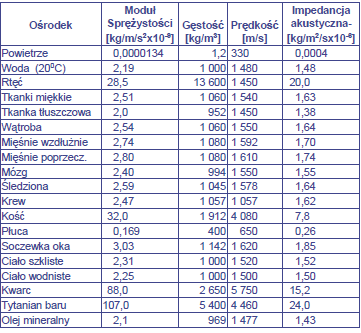
\includegraphics[width=0.55\textwidth]{figures/USG-params.png}
	\caption{Parametry ośrodków często mierzonych w badaniach USG.}
	\label{USG-params}
\end{figure}

Dla przykładu, do zjawiska załamania lub odbicia dochodzi kiedy fala pada na granice dwóch ośrodków o różnych impedancjach akustycznych $Z_1$ i $Z_2$. Dla fali prostopadłej zależność ta opisana jest następująco:
\begin{equation}
R = \frac{I_r}{I_0} = \left(\frac{Z_1-Z_2}{Z_1+Z_2}\right)^2,
\end{equation}
gdzie $I_r$ to natężenie fali padającej, a $I_0$ odbitej. Natomiast $R$, czyli współczynnik odbicia, jest parametrem, który rośnie wraz ze wzrostem kąta odchylenia od kierunku prostopadłego, aż do całkowitego odbicia.

Z kolei do rozpraszania bądź pochłaniania fali dochodzi kiedy to fala pokonuje daną drogę w ośrodku o pewnej $Z$, co zapisywane jest następująco:
\begin{equation}
I=I_0 \epsilon^{-\gamma x},
\end{equation}
gdzie $\gamma$ to współczynnik osłabienia zależny od $Z$, a $x$ to droga przebyta przez falę. Efekt ten można korygować poprzez dobór odpowiedniego $I_0$.

Analiza amplitudy i częstotliwości sygnału nadanego i echa umożliwia rekonstrukcję obrazu USG. W przypadku najczęściej stosowanych w praktyce rekonstrukcji przekrojów dwuwymiarowych (tzw. \textit{tryb B}) współczesny tor budowania prezentacji wizualnej (tzw. \textit{beamforming}) wygląda następująco: 
\begin{enumerate}
	\item Głowica ultradźwiękowa emituje impulsy w postaci wąskiej wiązki w ściśle określonym kierunku. Wiązka jest efektem interferencji sygnału z $N$ przetworników zawierających kryształy piezoelektryczne.
	\item Echa z danego kierunku pozwalają na obliczenie pojedynczego promienia akustycznego, który jest iloczynem charakterystyk nadawanego i odbieranego sygnału.
	\item Wszystkie promienie, których we współczesnych aparatach może być do kilkuset (zob. [GE Voluson]), służą do formowania obrazu, który tworzony jest we \textit{współrzędnych biegunowych} ($r$, $\theta$) w przypadku głowic mechanicznych sektorowych, wieloelementowych convex czy fazowych lub we współrzędnych prostokątnych ($x$, $y$) w przypadku głowic mechanicznych lub wieloelementowych liniowych\footnote{szczegółowy opis głowic USG i ich charakterystyk można znaleźć w []}. 
\end{enumerate}

Tryb B umożliwia również wizualizację obrazów dynamicznych. Przykładowo jeżeli na obraz składa się 400 promieni i każdy odsłuchiwany jest do głębokości 15 cm, to czas gromadzenia danych dla ośrodka o średnim c=1500 m/s wynosi $2\frac{2\times15}{1500 m/s}\times400 = 0,08 s$, czyli 12 obrazów na sekundę. Częstotliwość tę można zwiększać, zmniejszając liczbę promieni lub głębokość obserwacji.

Innym często stosowanym trybem rekonstrukcji obrazu jest \textit{tryb D} bazujący na \textit{efekcie Dopplera}, do którego dochodzi w przypadku przechodzenia fali przez ośrodek przesuwający się względem głowicy. Zmienia się wówczas częstotliwość fali, co wyrażone jest następującym wzorem:
\begin{equation}
f_r = 2 f_o\frac{v}{c}\cos(\theta),
\end{equation} 
gdzie $f_r$ to zmiana częstotliwości fali nadawanej $f_0$, zależna od kąta $\theta$ pomiędzy falą i ośrodkiem poruszającym się z prędkościami rozchodzenia się fali w obu ośrodkach tj. $v$ i $c$. Dla przykładu, im większa prędkość komórek przesuwających się w monitorowanym ciele pacjenta, tym większa jest $f_r$. Dlatego tryb D z powodzeniem jest wykorzystywany np. do monitorowania przepływu krwi w dużych naczyniach takich jak tętnice.

Rozwinięciem trybu D jest tryb \textit{Power D} (od ang. \textit{Power Doppler}). Gdzie zamiast przesunięcia częstotliwości interpretowana jest \textit{moc sygnału} Dopplerowskiego, czyli strata energii w zadanym czasie. Zależność mocy od częstotliwości nazywana jest \textit{widmem mocy sygnału}. Za pomocą odpowiedniego parametru nazywanego \textit{gain} można interpretować zadany wycinek widma, co sprawia, że możliwa staje się informatywna prezentacja przepływu o niskich prędkościach w niewielkich naczyniach takich jak naczynia włosowate. Dokładniej, tryb Power D ma nawet trzykrotnie większą czułość niż standardowy tryb D \cite{Babcock1996}.

W kontekście ścięgna Achillesa tryb Power D może służyć do oceny unaczynienia ścięgna w kolejnych etapach gojenia, które jak wiadomo z sekcji \ref{gojenie} zmienia się w czasie. Tryb B natomiast może być użyteczny do obrazowania struktury tkanek miękkich. W praktyce wykorzystywana jest zwłaszcza możliwość zobrazowania ukierunkowania struktur włókien ścięgnistych na podstawie czego radiolog może wnioskować o fazie gojenia. Składowa czasowa jest interesująca z perspektywy m.in. fizjoterapeuty oceniającego ślizg w ścięgnie przy wykonywaniu odpowiednich ruchów np. zginania podeszwowo-grzbietowego stopy. 

W porównaniu do rezonansu magnetycznego, w kwestii ograniczeń, należy zwrócić uwagę na fakt, że fale akustyczne używane w USG nie propagują się dobrze przez kości i gazy. Dlatego RM jest częściej rekomendowany do oceny struktur umiejscowionych w otoczeniu lub składających się w większości z takich ośrodków np. płuca. 

Z użyciem RM możliwe jest uzyskanie obrazów o lepszej jakości detali. Sam czas badania jest natomiast dłuższy i w większości przypadków niemożliwe jest obrazowanie w czasie rzeczywistym, co z kolei jest naturalne dla techniki USG.

W wymiarze finansowym istotny jest fakt, że aparat do USG kosztuje nawet 10 razy mniej niż aparatura do RM. Jak wspomniano jednak, z uwagi na jakość detali, uzyskiwane obrazy są trudniejsze do interpretacji, co przekłada się na koszty wyszkolenia kadry. 

W tym ostatnim kontekście przydatne mogą okazać się nowe rozwiązania w warstwie sprzętowej i oprogramowania. Do pierwszej grupy należy zaliczyć zastąpienie przetworników z piezoelektrykami, przetwornikami budowanymi w technologi MEMS np. cMUT, czy pMUT (zob. \cite{Butterfly2018}) oraz układy pozwalające przetwarzać surowy sygnał ultradźwiękowy (zob. \cite{US4US}). Dzięki przetwornikom MEMS można wytworzyć cały układ generujący drgania w krzemie w jednym procesie technologicznym razem z dedykowanym układem do zadanej aplikacji (ang. \textit{Application-Specific Integrated Circuit} w skr. \textit{ASIC}). Takie podejście znacząco redukuje koszty oraz implikuje możliwość miniaturyzacji urządzeń.

Do drugiej grupy należą algorytmy sztucznej inteligencji pozwalające wydobyć i zinterpretować interesującą informację z niskiej jakości obrazów. Przykładowo w \cite{Cunningham2017} algorytmy sztucznej inteligencji zostały użyte do określenia orientacji włókien mięśniowych, a w \cite{NVIDIA-CLARA} do segmentacji komór serca w czasie rzeczywistym. 

Obiecujący jest też rozwój metod charakterystyki tkanki na podstawie ultrasonografii (ang. Ultrasonography Tissue Characterization, w skr. \textit{UTC}). W 2003 r., w \cite{Bakker2003}, Bakker et. al. przedstawili pracę pokazującą w jakim stopniu obraz USG jest mieszanką echa związanego z budową tkanki, a w jakim z \textit{interferencji}, czyli nakładania się fal. W zależności od stabilności echa można zatem wnioskować czy obserwowana struktura składa się głównie z dużych, stałych struktur wywołujących stabilne echo, czy np. płynów lub małych włókienek powodujących zmienne interferencje. Jako referencji dla studiowanego echa używa się badań histologicznych (zob. \cite{Bakker2000}). Na tej podstawie sklasyfikowano 4 różne rodzaje echa i jak zasygnalizowano w pracach \cite{vanSchie2009} i \cite{Heyward2018} informacja o proporcjach występowania tych rodzai może być użyta do oceny struktury ścięgna Achillesa. Metoda ta nie została jednak jeszcze w pełni zwalidowana i możliwości wnioskowania na jej podstawie są wciąż niejasne (zob. \cite{Heyward2018}).

USG i inne techniki obrazowania medyczne nie są jedynymi metodami oceny gojenia się ścięgna Achillesa. W kolejnej sekcji zostały opisane techniki oceny funkcji ścięgna, które samodzielnie jak i w połączeniu z analizą obrazową stanowią wartościową informację diagnostyczną.

\section{Zastosowanie badań biomechanicznych}

W poprzednich sekcjach zostały opisane dwie najczęstsze obrazowe metody monitorowania procesu gojenia się ścięgna Achillesa z udziałem badań obrazowych pozwalających na ocenę struktury tkanki. Komplementarnie, podczas rehabilitacji może być również wykonana \textit{ocena funkcjonalna}, technika weryfikująca w jakim stopniu dany element (tkanka, narząd, organizm) może realizować swoje zadania. W przypadku monitorowania gojenia się ścięgna Achillesa najczęściej w tym celu stosuje się \textit{ocenę biomechaniki}, czyli badania pozwalające wnioskować na temat właściwości mechanicznych elementów składowych organizmów żywych. 

Najbardziej zaawansowane i dokładne metody oceny biomechaniki stosowane współcześnie możliwe są do wykonania przy użyciu urządzeń pomiarowych takich jak:
\begin{itemize}
	\item \textit{Komputerowa analiza ruchu} (ang. \textit{Motion Capture}) -- narzędzie wykorzystujące systemy czujników do zapisu informacji o zmianach położenia obiektu rejestrowanego np. pacjenta. Do wiodących rozwiązań należy zaliczyć systemy firmy Vicon \cite{Vicon}, czy BTS \cite{BTS}.
	\item \textit{Płyty dynamometryczne} (ang. \textit{Force Plates}) -- narzędzie wykorzystywane do pomiaru sił reakcji podłoża w trzech prostopadłych płaszczyznach. Dzięki temu można określić sumaryczny udział mięśni w generowaniu sił odpowiadających za balans ciała, ruch w danym kierunku oraz przeciwstawianie się sile grawitacji. Do wiodących rozwiązań należą płyty firmy Kistler \cite{KISTLER}.
	\item \textit{Elektromiografia}, w skr. EMG (ang. \textit{Electromyography}) -- narzędzie do pomiaru pobudzeń poszczególnych grup mięśniowych podczas ruchu. Wykorzystywane jest m.in. do określenia rozkładu sił zmierzonych przez płyty dynamometryczne na poszczególne mięśnie.
\end{itemize}

Synchronizacja danych z powyższych urządzeń umożliwia konstrukcję modeli układu mięśniowo-szkieletowego i symulacje funkcji poszczególnych grup mięśniowych lub ścięgien przy zadanych problemach.

Danymi stosowanymi do uszczegółowienia takich modeli są np.: wymiary poszczególnych segmentów ciała (goleń, udo, tors) tzw. pomiary antropometryczne; maksymalne siły izometryczne mierzone z użyciem systemów takich jak Biodex; geometria kości mierzonych np. z pomocą tomografii komputerowej (w skr. TK) ew. RM; lokalizacja przyczepów mięśniowych określanych przy pomocy MR lub USG; środki masy poszczególnych segmentów określanych np. przy użyciu badania \textit{DXA} (od ang. \textit{Double X Ray Absorption}); skład włókien mięśniowych widocznych w USG.

Z uwagi na dużą liczbę możliwych do zmierzenia parametrów, ich integracja odbywa się w modelach komputerowych zaimplementowanych w różnego rodzaju oprogramowaniu do symulacji biomechanicznych. Do najczęściej używanych modeli należą opisane w \cite{John2013} Gait2392, Gait 2354 oraz obecnie najbardziej złożony -- \textit{AnyBody Full Body Model} \cite{Bassani2017}. 

Historia komputerowo wspomaganego, kompleksowego modelowania biomechaniki ruchu sięga wczesnych lat 90-tych ubiegłego wieku, kiedy to Delp i Loan przedstawili oprogramowanie SIMM \cite{Delp1990}. Obecnie SIMM jak również inne oprogramowania komercyjne takie jak: Visual 3D (Cmotion Inc.) \cite{Visual3D}, Anybody (Anybody Technology) \cite{AnyBody}, czy Adams (MSC Software Corp.) \cite{Adams}, dostarczają narzędzi do wartościowych symulacji np. chodu \cite{Steele2010}, biegu \cite{Hamner2010} jak również konsekwencji różnych zabiegów chirurgicznych \cite{Gomes2013} i chorób \cite{Shao2009}. Istnieją również narzędzia otwarte, do których należą szeroko wykorzystywany OpenSim \cite{Delp2007} rozwijany na Uniwersytecie w Stanford, czy też Human Motion \cite{Riken} wywodzący się z instytutu badawczego RIKEN w Japonii.

Powyżej przedstawione kompleksowe badania w praktyce realizowane są rzadko z uwagi na wysokie koszty. Dla przykładu w Polsce, ośrodki wyposażone w sprzęt pomiarowy takiej klasy to np. Instytut "Pomnik – Centrum Zdrowia Dziecka", Warszawski Uniwersytet Medyczny, Akademia Wychowania Fizycznego imienia Józefa Piłsudskiego, czy komercyjna placówka Fizjofit w Gliwicach. Żeby obniżyć koszty badania stosuje się wybiórcze podejście i selekcję parametrów pomiarowych uznanych przez ekspertów dziedzinowych za wystarczające do analizy zadanego problemu. Dla przykładu badania stosowane do oceny biomechaniki ścięgna Achillesa w placówce Carolina Medical Center (gdzie realizowane były badania wykorzystywane w tej pracy) składają się z następujących pomiarów (zob. \cite{CMC}):

\begin{enumerate}
	\item Pomiar \textit{ATRS} (od ang. \textit{Achilles Tendon Total Rupture Score}) -- oceniany jest w skali od 0 do 100 [Nilsson-Helander i wsp. 2007, Bąkowski i wsp. 2017] poziom ograniczenia, z którymi pacjenci borykają się w następstwie urazu.
	\item Pomiar stabilograficzny na platformie dynamometrycznej -- mierzone są wychylenia środka ciężkości. Pacjent ma za zadanie utrzymanie równowagi na niestabilnym podłożu. Badanie realizowane jest boso z oczami otwartymi. Wykonane są dwie próby po 30 sekund kolejno na prawej i lewej kończynie dolnej na dynamicznej platformie dynamometrycznej Biodex Balance System. Wyniki zostają porównane między kończynami. 
	\item Pomiar stabilograficzny na platformie statycznej -- mierzona jest droga wychylenia środka masy pacjenta w trakcie stania jednonóż na platformie dynamometrycznej, statycznej.
	\item Pomiar sił reakcji na ścieżce podometrycznej -- mierzony jest rozkład sił nacisków podeszwowej strony stóp na podłoże (jedynie w kierunku prostopadłym do podłoża). Pomiar wykonywany jest podczas stania swobodnego, wspięć na palce oraz przysiadu boso bez odrywania pięt. Dokonywana jest również analiza chodu (3 przejścia) i biegu (5 przebiegnięć). Boso oraz w obuwiu sportowym. Na podstawie sił reakcji wyliczane są parametry: rotacja podudzia [deg], długość kroków [cm], udział fazy podparcia [\%], udział fazy przenoszenia [\%], maksymalna siła na pięcie [N] oraz maksymalna siła na palcach [N].
	\item Pomiar skoczności i mocy (tzw. siły dynamicznej) kończyn dolnych -- mierzona jest moc maksymalna $P_{max}$ i średnia $P_m$, maksymalna wysokość uniesienia $h_{max}$ i obniżenia $k$ środka masy ciała przed odbiciem. Wykonywane są wyskoki pionowe z miejsca na platformie dynamometrycznej. Realizowane są dwie próby obunóż oraz na prawej i lewej kończynie dolnej w obuwiu sportowym. W celu pełnego zaangażowania kończyn dolnych pacjent podczas badania trzyma ręce na biodrach. 
	\item Pomiary momentów sił mięśni stawu skokowego -- mierzone są maksymalne wartości momentu siły mięśni zginaczy podeszwowych i grzbietowych stawu skokowego [Nm] oraz deficyt pomiędzy operowaną i zdrową kończyną dolną [\%]. Momenty sił mierzone są w dwóch pozycjach tj. z wyprostowanym oraz zgiętym do 50 stopni stawem kolanowym [Orishimo i wsp. 2008]. Pomiar realizowany jest w warunkach izometrii i izokinetyki w trzech prędkościach kątowych 60$^\circ$/s (5 powtórzeń), 120$^\circ$/s (8 powtórzeń) oraz 180$^\circ$/s (10 powtórzeń) przy wykorzystaniu urządzenia Humac Norm (USA). Przed badaniem osoba odbywa 5 minutową rozgrzewkę na steperze.
\end{enumerate}

Wymienione wyżej badania zostały określone przez ortopedów i fizjoterapeutów jako wystarczające do oceny przywracania funkcji ścięgna Achillesa po rekonstrukcji. 

Wraz z oceną strukturalną realizowaną poprzez badania obrazowe i wiedzą ekspercką informacja tak zgromadzona może służyć do subiektywnego monitorowania procesu gojenia się ścięgna. Do skutecznej obiektywizacji tego procesu potrzebne są jednak dodatkowe metody bazujące na agregacji ilościowych współczynników i automatycznym wnioskowaniu na ich podstawie. Do tej grupy należą algorytmy sztucznej inteligencji opisane w kolejnym rozdziale. 